\documentclass[letterpaper]{article}

\usepackage[T1]{fontenc}
\usepackage{natbib}

\usepackage{geometry}

\usepackage{microtype,graphicx,booktabs,amsmath,caption}
\usepackage[hidelinks]{hyperref}

\geometry{margin = 1in}
\usepackage{setspace}

% \usepackage[style = chem-acs]{biblatex}
% \addbibresource{references.bib}

% \usepackage[
%   backend=biber,
%   style=chem-acs
% ]{biblatex}
% \addbibresource{references.bib}

% If you are using classical BibTeX, remove the above lines and 
% uncomment:
%\usepackage{achemso}

%%%%%%%%%%%%%%%%%%%%%%%%%%%%%%%%%%%%%%%%%%%%%%%%%%%%%%%%%%%%%%%%%%%%%
%% Graphic inclusion and scheme and chart support
%%%%%%%%%%%%%%%%%%%%%%%%%%%%%%%%%%%%%%%%%%%%%%%%%%%%%%%%%%%%%%%%%%%%%
\usepackage{graphicx}
\usepackage{float}
\newfloat{scheme}{htbp}{los}
\floatname{scheme}{Scheme}
\floatname{chart}{Chart}
\newfloat{graph}{htbp}{loh}

%%%%%%%%%%%%%%%%%%%%%%%%%%%%%%%%%%%%%%%%%%%%%%%%%%%%%%%%%%%%%%%%%%%%%
%% Common support packages
%%%%%%%%%%%%%%%%%%%%%%%%%%%%%%%%%%%%%%%%%%%%%%%%%%%%%%%%%%%%%%%%%%%%%
\usepackage{chemformula} % Formulas using \ch{}
% or
\usepackage[version = 4]{mhchem} % Formulas using \ce{}
\usepackage{amsmath}
\usepackage{amssymb}

%%%%%%%%%%%%%%%%%%%%%%%%%%%%%%%%%%%%%%%%%%%%%%%%%%%%%%%%%%%%%%%%%%%%%
%% Many journals require that sections are unnumbered: this 
%% is activated here
%%%%%%%%%%%%%%%%%%%%%%%%%%%%%%%%%%%%%%%%%%%%%%%%%%%%%%%%%%%%%%%%%%%%%
\setcounter{secnumdepth}{-1}

%%%%%%%%%%%%%%%%%%%%%%%%%%%%%%%%%%%%%%%%%%%%%%%%%%%%%%%%%%%%%%%%%%%%%
%% Place any additional macros here.  Please use \newcommand* where
%% possible, and avoid layout-changing macros (which are not used
%% when typesetting).
%%%%%%%%%%%%%%%%%%%%%%%%%%%%%%%%%%%%%%%%%%%%%%%%%%%%%%%%%%%%%%%%%%%%%
\newcommand*\mycommand[1]{\texttt{\emph{#1}}}

%%%%%%%%%%%%%%%%%%%%%%%%%%%%%%%%%%%%%%%%%%%%%%%%%%%%%%%%%%%%%%%%%%%%%
%% Author and title data:
%% the authblk package is currently the simplest way to provide this
%%%%%%%%%%%%%%%%%%%%%%%%%%%%%%%%%%%%%%%%%%%%%%%%%%%%%%%%%%%%%%%%%%%%%
\usepackage{authblk}
\author{Anonymous Authors}
\title{Learning Molecular Response Landscapes Across Bioassays}
\date{}

% \usepackage[
%   backend=biber,
%   style=chem-acs
% ]{biblatex}

% \addbibresource{references.bib}


\begin{document}
\maketitle
\graphicspath{{../outputs/figures/}}

% Generated from compiled Supplementary Information; run the reference audit after SI compilation.
\newcommand{\SIControlledTable}{S1}
\newcommand{\SIFinalTable}{S2}


\begin{abstract}
Reliable cross-assay structure--activity relationships (SAR) are essential for analogue selection in medicinal chemistry. However, changes in assay conditions can alter both absolute potency and relative compound ordering. Existing assay-aware activity predictors do not directly distinguish loss of an analogue ordering from a molecule's departure from the common assay shift. We address these questions through two prediction tasks within known assay pairs: SAR transfer and molecular sensitivity. A curated ChEMBL37 benchmark contains 79,810 paired molecular observations and 73,950 eligible analogue comparisons. We introduce SAGP (SAR-Aware Gaussian Process), a lightweight model that conditions on historical compounds measured in both assays. SAGP combines a structured potency response with local chemical variation to estimate individual molecular responses, analogue contrasts and associated risks. Across five scaffold splits, SAGP achieves SAR-transfer AP of 0.539 and within-pair AUROC of 0.746, and molecular-sensitivity AP of 0.644 with macro MAE of 0.160 pIC$_{50}$. Shuffling historical molecule--response associations reduces sensitivity within-pair AUROC from 0.697 to 0.527, showing that matched molecular responses provide useful information beyond an assay-wide shift. These results support chemical risk prioritization for assay transitions with historical paired measurements.
\end{abstract}

\section{Introduction}

Medicinal chemistry depends on reliable comparisons between compounds. An apparent potency gain guides analogue synthesis and compound selection only if the experimental comparison remains meaningful as a program moves between assays. IC$_{50}$ is an operational endpoint whose relationship to affinity depends on substrate concentration and reaction kinetics \citep{cheng1973ic50}. Changes in protein preparation, incubation, medium or readout can therefore alter the measured response. When a chemical series is tested in different systems, the practical question is whether its SAR conclusions remain useful and which compounds require additional measurement.

Public bioactivity databases provide the paired measurements needed to study this question, but also expose substantial heterogeneity. Landrum and Riniker found considerable cross-source disagreement in IC$_{50}$ and $K_i$ values, including variation remaining after restrictive filtering \citep{landrum2024noise}. Analyses by Kramer and colleagues and subsequent public-data studies likewise distinguish heterogeneous-source uncertainty from repeated in-house assay variability \citep{kramer2012uncertainty,kalliokoski2013mixed,kramer2016variability}. A shared assay shift can change absolute potencies while preserving analogue ordering; compound-specific departures can instead attenuate or reverse an apparent structural benefit. Cross-assay matched-pair analyses suggest that relative activities can be more stable than absolute values \citep{nelen2025matched}, motivating a separation of these two effects.

Assay-aware prediction incorporates experimental context into molecular learning. Schoenmaker et al. used assay-description representations to improve proteochemometric prediction \citep{schoenmaker2025context}; CLAMP and TwinBooster combine molecular and assay-language information, while AssayMatch selects compatible training assays \citep{seidl2023clamp,schuh2024twinbooster,fan2026assaymatch}. Low-data methods use measured support compounds: FS-Mol and CARA define assay-centered benchmarks, and MHNfs and ActFound learn contextual or relative activity relationships \citep{stanley2021fsmol,tian2024cara,schimunek2023mhnfs,feng2024actfound}. These approaches typically predict activity in an assay. Predicting whether a chemical conclusion survives a particular assay transition requires an additional comparison between the two measurement systems.

Local SAR provides a useful basis for that comparison. Activity-cliff and nonadditivity studies characterize large potency changes between related structures and show that aggregate prediction accuracy can conceal local errors \citep{hu2012mmpcliffs,stumpfe2014cliffs,dimova2016cliffs,stumpfe2019concept,nonadditivity2021,tilborg2022cliffs}. Molecular GPs connect chemical similarity to continuous responses and uncertainty; nearest-neighbor GPs, Tanimoto random features and learned-kernel methods extend this framework \citep{difranzo2020nngp,tripp2023tanimoto,wilson2016dkl,patacchiola2020dkt,chen2023adkf}. These ingredients support two distinct targets that pointwise potency accuracy does not directly evaluate: loss of an analogue ordering across assays, and an individual molecule's departure from the common assay shift. Historical compounds measured in both assays offer an empirical description of the transition even when explicit protocol annotations are sparse.

We define these targets as SAR transfer (Task 1) and molecular sensitivity (Task 2) within supported, known assay pairs. A source-traceable ChEMBL37 benchmark retains 79,810 paired molecular observations and 73,950 eligible analogue comparisons. SAGP (SAR-Aware Gaussian Process) combines a structured potency-axis response with chemically local residual variation, conditions on historical paired measurements, and supplies individual-response and analogue-contrast estimates to small decision adapters. The 1,883-parameter model predicts both event risks and continuous quantities while keeping query assay-B measurements hidden. Figure~\ref{fig:pipeline} summarizes the workflow.

Across five scaffold splits, the model reaches SAR-transfer AP 0.539 and within-pair AUROC 0.746, and sensitivity AP 0.644 with macro MAE 0.160 pIC$_{50}$. Shuffling historical compound--response associations reduces sensitivity within-pair AUROC from 0.697 to 0.527. These two findings establish useful prediction within represented assay transitions and identify molecularly matched reference responses as an important source of information. The results connect useful molecular predictions to the measured responses of historical compounds.

\begin{figure}[t]
\centering
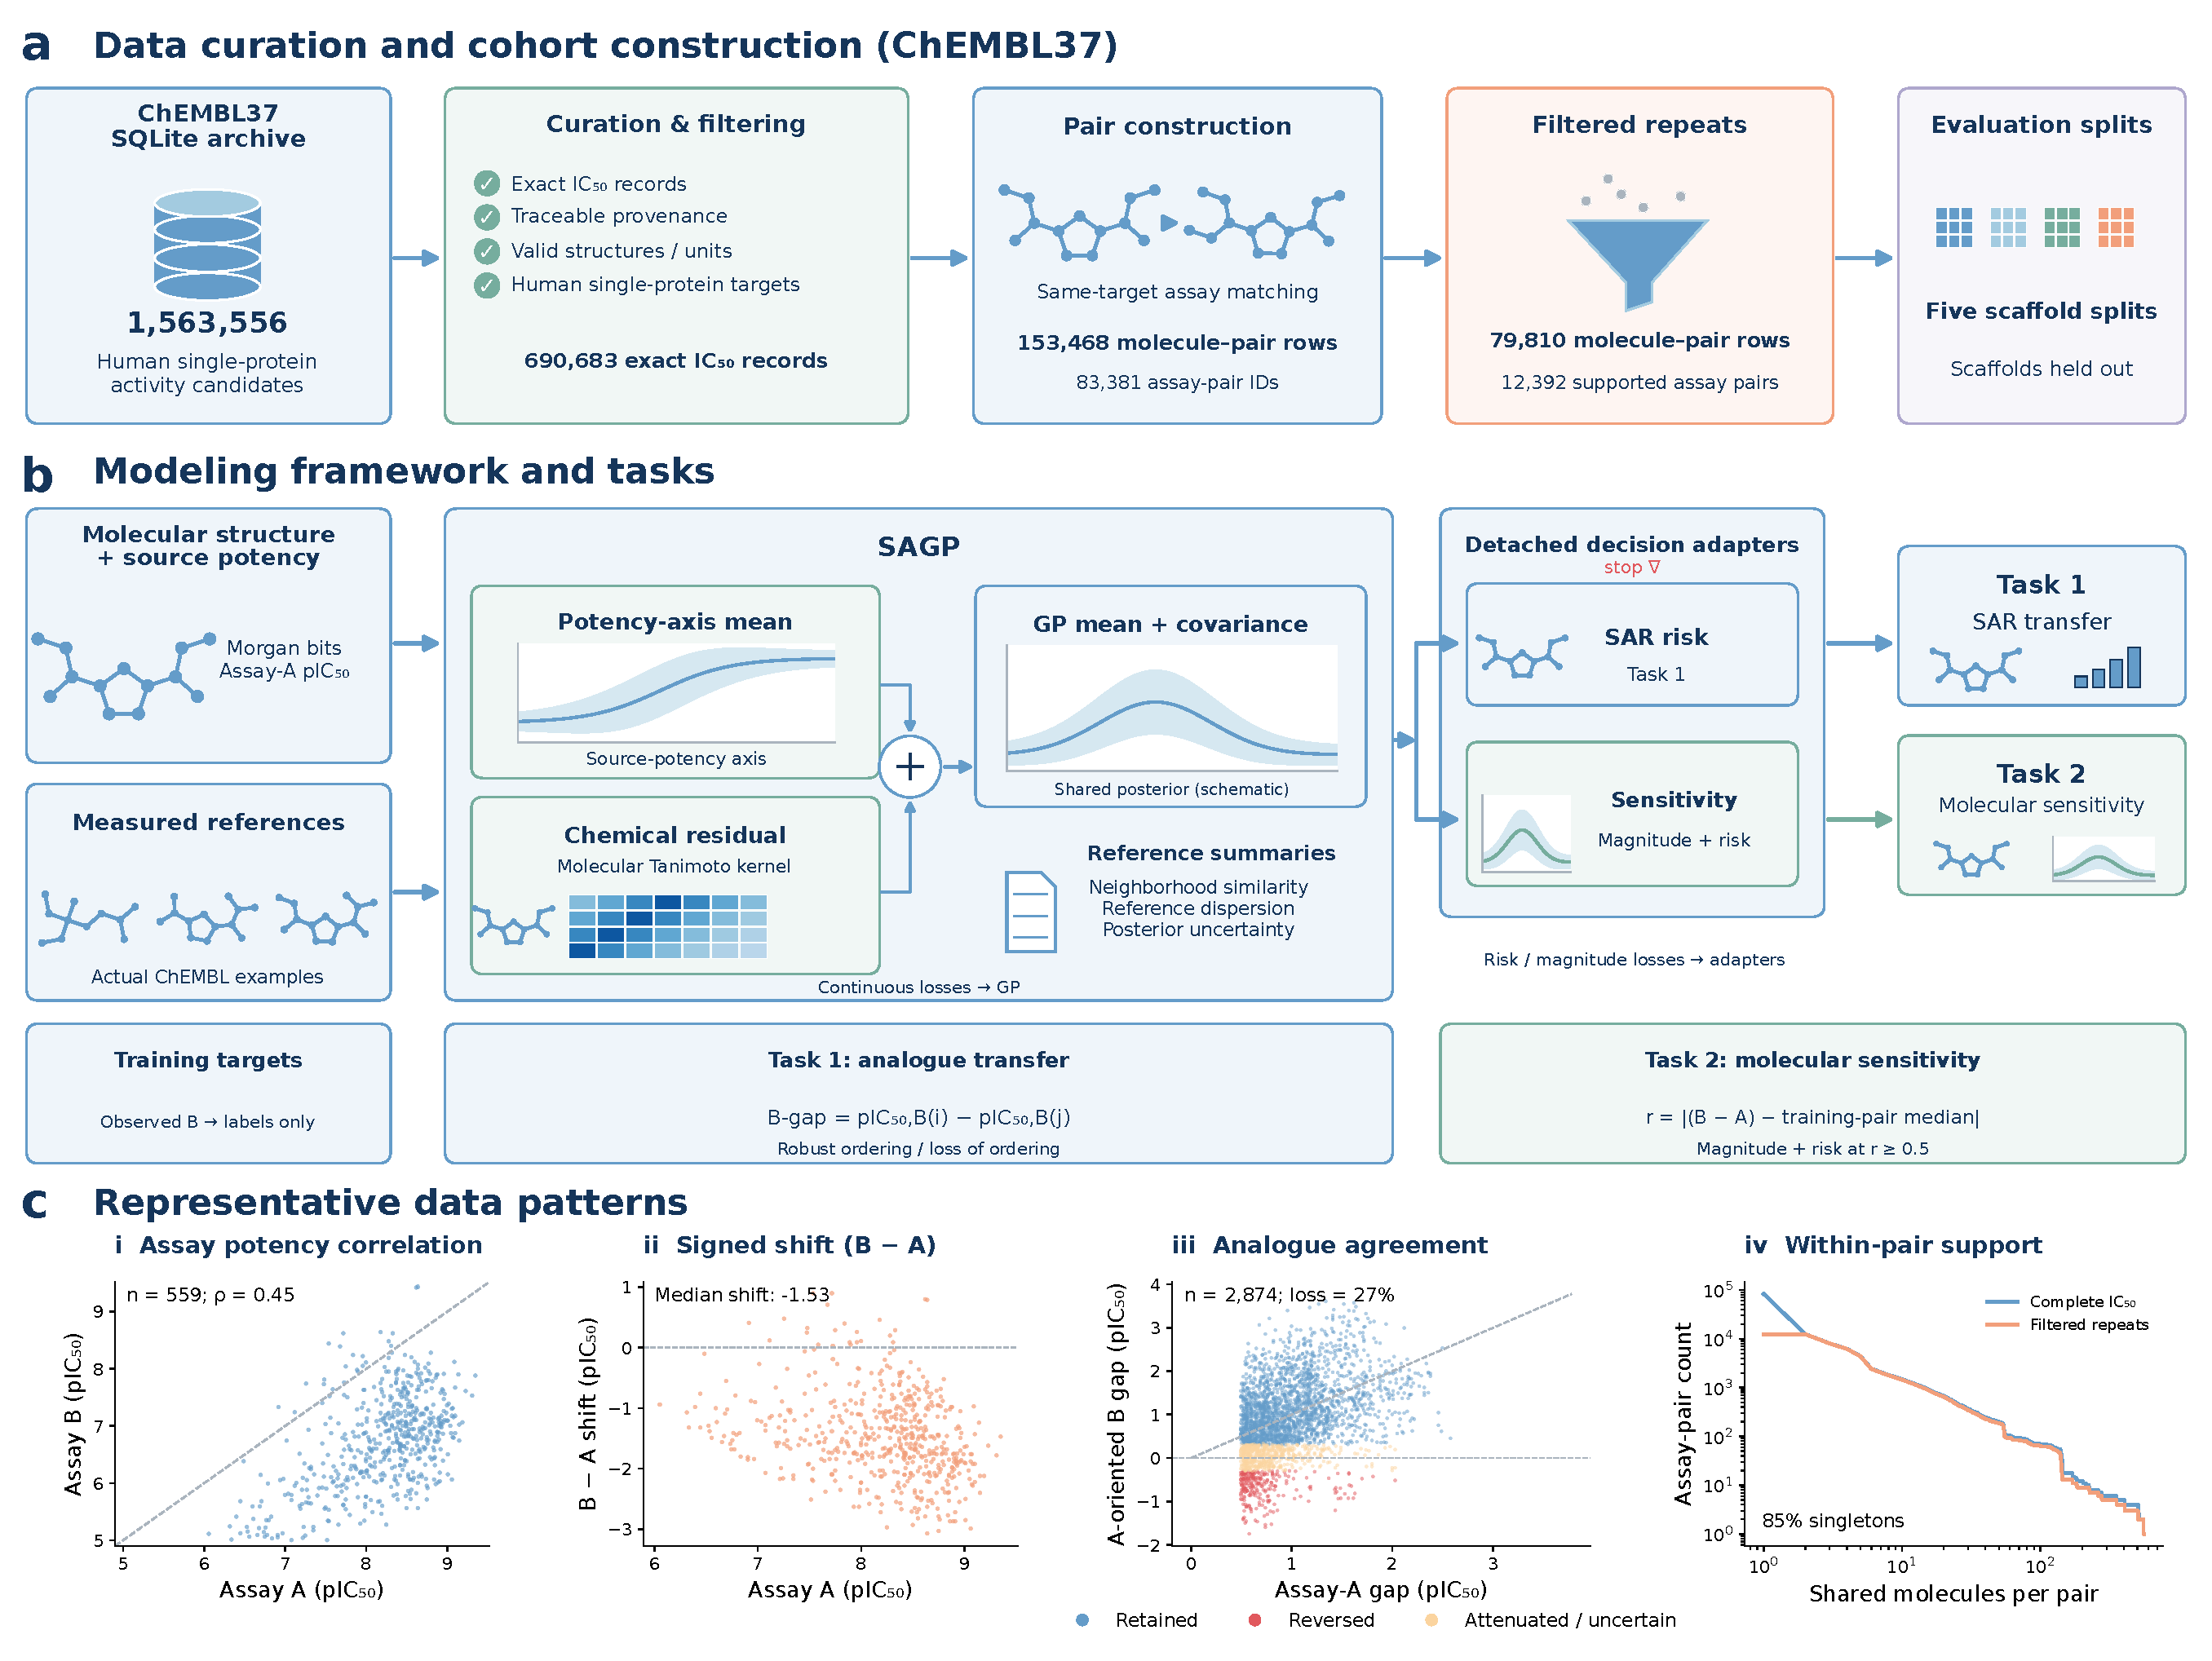
\includegraphics[width=\textwidth]{figure1_pipeline.pdf}
\caption{Data selection, SAGP and observed response patterns. (a) Extraction, exact IC$_{50}$ selection, same-target pairing, provenance filtering and analogue construction use distinct counting units. Evaluation uses five scaffold splits for known assay pairs. (b) Structures, assay-A potencies and measured references condition a monotone mean and molecular Tanimoto residual. One shared posterior supplies continuous moments to detached decision adapters for Tasks 1 and 2. Continuous contrast/root losses update the GP; binary and magnitude losses update their respective adapters. The lower strip distinguishes the two training targets; observed query-B values are labels and never prediction inputs. Query assay-B values remain hidden. (c) Observed-data panels: (i) paired potencies and (ii) signed response shifts for the largest supported assay pair (559 molecules), selected by support alone; (iii) all 2,874 eligible analogue comparisons in that pair show retained, reversed or attenuated/uncertain ordering; (iv) support survival curves count assay pairs with at least the stated number of shared molecules before and after filtering. The 153,468 and 79,810 counts are molecule--assay-pair rows, not assay-pair identities. Molecular icons are schematic connectivity diagrams derived from validated ChEMBL structures, with atom identities and bond orders abstracted; response curves are schematic and the bottom panels use actual observations.}
\label{fig:pipeline}
\end{figure}

\section{Materials and Methods}

\subsection{Curation and traceable pair construction}

We used the local ChEMBL37 SQLite archive and retained its extraction and curation audit \citep{papadatos2015curation,mendez2019chembl,chembl2023,chembl37}. Of 1,563,556 human single-protein activity candidates, 916,331 passed the rules: 690,683 exact IC$_{50}$ and 225,648 Ki records. Exclusions remove non-exact relations, potential duplicates, non-binding assay types, validity flags, recorded cell/organism context, invalid structures, and invalid values or units. Ki is recorded in the inventory but is not modeled in this study. Missing protocol metadata are not imputed as experimental facts.

Structures were standardized to stereo-preserving parents, consistent with the separation of chemical-identity checks from activity curation \citep{fourches2010curation,fourches2016curation,kalliokoski2013quality}. Validated concentrations were converted to $pIC_{50}=-\log_{10}(IC_{50}\,[\mathrm{M}])$. Replicates were summarized within the same molecule--\allowbreak target--\allowbreak endpoint--\allowbreak assay group while retaining their ranges and contributing activity identifiers. Pairing a molecule measured in assays A and B of the same target produces a molecule--assay-pair observation. The complete IC$_{50}$ resource contains 153,468 such observations over 83,381 assay pairs (Table~\ref{tab:data-resource}). Removing 2,742 rows with shared source provenance and requiring at least two remaining shared molecules per pair yields the 79,810-observation pool used for response modeling. Molecules, assays and source documents remain traceable throughout.

\begin{table}[!htbp]
\centering
\caption{Data resource and task cohorts. Rows have different observation units and are not additive. Retained activity records comprise IC$_{50}$ and Ki; only IC$_{50}$ is modeled. The protocol audit is a separate descriptive cohort. Dashes indicate dimensions not separately tabulated.}
\label{tab:data-resource}
\small
\setlength{\tabcolsep}{4pt}
\resizebox{\textwidth}{!}{%
\begin{tabular}{llrrr}
\toprule
Dataset & Observation unit & Rows & Assay pairs & Targets \\
\midrule
SQL candidates & Activity record & 1,563,556 & -- & -- \\
Excluded by curation & Activity record & 647,225 & -- & -- \\
Retained exact records & Activity record & 916,331 & -- & 2,884 \\
Primary IC50 records & Activity record & 690,683 & -- & -- \\
Ki records (not modeled) & Activity record & 225,648 & -- & -- \\
Complete IC50 pairing & Molecule--assay pair & 153,468 & 83,381 & 1,414 \\
Provenance-filtered repeated pairs & Molecule--assay pair & 79,810 & 12,392 & 846 \\
Task 1 eligible cohort & Analogue comparison & 73,950 & 2,596 & 452 \\
Separate protocol audit & Sample--condition row & 4,626 & 1,008 & 179 \\
\bottomrule
\end{tabular}}
\end{table}


\subsection{Analogue eligibility, outcomes and source composition}

An analogue comparison uses two molecules measured in the same assay pair, supported by four distinct activity records. Task 1 requires Morgan Tanimoto similarity $\geq0.70$ \citep{rogers2010ecfp}, a robust assay-A gap $\geq0.5$ pIC$_{50}$, and at least five shared molecules per assay pair. Assay-B values assign outcomes and never determine eligibility or query features. Retention requires the same ordering with a robust B-gap $\geq0.3$; SAR loss includes reversal, attenuation or replicate-range uncertainty. The resulting eligibility cohort is summarized in Table~\ref{tab:data-resource}; outcome distributions are reported in Results and Discussion.

A separate protocol audit summarizes numeric and categorical condition mentions in assay descriptions. Effective exposure may depend on protein binding or aggregation \citep{trainor2007proteinbinding,mcgovern2002detergent,feng2018colloidal}, and product inhibition can affect chromogenic readouts \citep{stobb2019chromogenic}; these motivate condition annotation without assigning a cause to individual observed shifts.

\subsection{Two prediction tasks}

\paragraph{Task 1: SAR transfer within a known assay pair.} Given a similar molecular pair, assay-A potencies, structures and allowed historical training references, estimate whether the assay-A ordering remains robust in assay B. The primary binary label marks reversal, attenuation or uncertainty as a loss. The continuous target is the median assay-B potency gap. Query assay-B outcomes are never model inputs. Comparisons sharing molecules, assay pairs or sources are dependent; the five scaffold partitions are repeated evaluations, not independent biological replications.

\paragraph{Task 2: molecular sensitivity within a fixed assay pair.} For molecule $m$, define its signed response shift $d(m)=pIC_{50,B}(m)-pIC_{50,A}(m)$. The task target is the absolute residual $r(m)=|d(m)-\widetilde d_{pair}|$, where $\widetilde d_{pair}$ is the median shift estimated from training molecules in that pair only. We predict both $r(m)$ and whether it reaches 0.5 pIC$_{50}$. Pairs require at least 30 training molecules; query scaffolds, measurements and provenance groups are excluded from their support pools.



\subsection{Evaluation partitions}

Five fixed seeds (17, 23, 41, 71 and 101) define repeated scaffold-held-out partitions, following structural-group evaluation of chemical generalization \citep{murcko1996,sheridan2013timesplit,wallach2018memorization}. Large-scale molecular benchmarks likewise show why endpoint composition and evaluation protocol should be specified together \citep{mayr2018prediction,wu2018moleculenet}. Both molecules of each analogue comparison must remain in one partition; crossing comparisons are removed. Task 1 additionally requires five training molecules and five training comparisons per assay pair; Task 2 requires 30 training molecules. Consequently, cohort sizes vary substantially by seed. Table~\ref{tab:task-cohorts} reports training, validation and test ranges, separately from the number of test pairs that meet the class-support rule for within-pair AUROC. Exact counts for every seed are supplied with the manuscript.

\begin{table}[!htbp]
\centering
\caption{Task-specific training, validation and test cohorts across five fixed seeds (17, 23, 41, 71, 101). Ranges describe repeated partitions, not independent replications. Test pairs count all represented assay pairs; evaluable pairs require at least ten queries and three examples per class, matching the strict ranking comparison in Fig.~\ref{fig:gains}a.}
\label{tab:task-cohorts}
\small
\setlength{\tabcolsep}{3.4pt}
\resizebox{\textwidth}{!}{%
\begin{tabular}{lrrrrr}
\toprule
Task and observation unit & Training rows & Validation rows & Test rows & \shortstack{Test\\pairs} & \shortstack{Evaluable\\pairs} \\
\midrule
\shortstack[l]{Task 1: SAR transfer\\(analogue comparisons)} & 31,781--48,941 & 1,258--2,071 & 1,705--13,688 & 182--297 & 17--55 \\[4pt]
\shortstack[l]{Task 2: Molecular sensitivity\\(molecule observations)} & 10,396--15,717 & 1,485--2,462 & 2,039--4,420 & 147--216 & 18--35 \\[4pt]
\bottomrule
\end{tabular}}
\vspace{3pt}
\begin{minipage}{0.98\textwidth}\footnotesize
Training rows count task-specific eligible examples, not gradient updates. Additional signed-shift supervision draws on 53,048--57,239 paired observations per seed before reference-support eligibility; this is not an additional independent cohort. Tasks 1 and 2 hold out query scaffolds within known pairs. Query measurements and provenance groups remain excluded from reference pools.
\end{minipage}
\end{table}


Additional signed-shift supervision is restricted to training scaffolds. Query measurements and provenance groups are excluded from their reference pools. Descriptor transformations, reference statistics and pair offsets are estimated from training data only.

\subsection{Inputs and a shared continuous response posterior}

For a directed assay transition A$\rightarrow$B, the input is a query structure and its known assay-A potency, plus historical references $S=\{(x_s,p_s,d_s)\}$ measured in both assays. Here $d_s=pIC_{50,B,s}-pIC_{50,A,s}$ and $p_s=(pIC_{50,A,s}-6)/2$. The query B potency is withheld. Structures enter this model through 2,048-bit, radius-2, chirality-aware Morgan fingerprints \citep{rogers2010ecfp}. The shared feature cache also contains eleven descriptors for other baselines; SAGP does not consume those descriptor columns. Neither target ESM embeddings nor assay IDs or parsed protocol variables are learned model inputs. Target identity restricts valid pairs; observed reference responses condition the transition. Thus the method represents an assay transition through measured behavior rather than requiring a dense catalogue of protocol categories.

Reference moments adjust covariance amplitudes and nine positive slopes in a smooth potency-axis response; monotonic and shared-output GP constructions provide related statistical tools \citep{riihimaki2010monotone,bonilla2008multitaskgp}. With reference mean $\bar p$, scale $s_p\geq0.25$ and $z=(p-\bar p)/s_p$, define
\begin{align}
 I_S(z)&=a_1z+\sum_{j=1}^{8}(a_{j+1}-a_j)\,0.15\log[1+\exp((z-\kappa_j)/0.15)],\\
 m_S(p)&=2s_p\{I_S(z)-I_S(0)-z\},\qquad a_j>0.
\end{align}
The eight knots are equally spaced from $-1.75$ to $1.75$. The implied prior assay-B potency trend is monotone, while molecule-specific residuals permit reversals. Reference summaries, positive-parameter transforms and numerical implementation are given in Supplementary Methods.

The GP posterior follows standard Gaussian conditioning \citep{rasmussen2006gp}; its molecular similarity component uses the Tanimoto coefficient on binary fingerprints, a common representation for local chemical similarity \citep{ralaivola2005kernels,difranzo2020nngp,tripp2023tanimoto}. The residual covariance is
\begin{equation}
 k_S((x,p),(x',p'))=\eta_0+\eta_{p,S}pp'+\eta_{T,S}\,T(x,x'),\qquad
 T(x,x')=\frac{x^\top x'}{|x|+|x'|-x^\top x'},
\end{equation}
with positive amplitudes and context-dependent observation noise $\sigma_S^2$. Reference context uses potency/shift moments and sample-count information, excluding query outcomes. For query set $Q$, standard Gaussian conditioning gives
\begin{align}
 \mu_Q&=m_Q+K_{QS}(K_{SS}+\sigma_S^2I+10^{-4}I)^{-1}(d_S-m_S),\\
 \Sigma_Q&=K_{QQ}-K_{QS}(K_{SS}+\sigma_S^2I+10^{-4}I)^{-1}K_{SQ}+\sigma_S^2I.
\end{align}
Cholesky solves are used rather than an explicit inverse. The added query noise makes this a predictive covariance for observed shifts. No separately fitted predictions are averaged.

\subsection{Task outputs from the response estimates}

For an assay-A-ordered analogue pair $(i,j)$, the assay-B gap has mean and variance
\begin{equation}
 \mu_g=\Delta p_A+\mu_i-\mu_j,\qquad
 v_g=\Sigma_{ii}+\Sigma_{jj}-2\Sigma_{ij}.
\end{equation}
This contrast accounts for shared uncertainty between the two molecules. The SAR event margin is $h_1=0.3+w_S-\mu_g$, where $w_S$ is the mean measured B replicate-range width among permitted historical references. For Task 2, the signed residual mean is $\mu_i-\widetilde d_{pair}$ and its predictive variance is $\Sigma_{ii}$.

Three small decision adapters produce SAR-loss risk $P_1$, sensitivity magnitude $q_i$ and sensitivity-event risk $P_2$. Each uses an $8\rightarrow12\rightarrow o$ SiLU network, with $o=2,2,1$, respectively. Inputs summarize the response moments, reference dispersion, source-potency position and molecular neighborhood. GP moments are detached before decision training; the sensitivity magnitude is additionally detached before event classification. Individual prediction scores are not ensembled. The full model stores 1,883 scalar parameters. The exact summary coordinates, folded-normal magnitude transformation and risk equations are specified in Supplementary Methods.

\subsection{Training and validation selection}

A root-shift-only pretrained response checkpoint initializes SAGP. The response component learns continuous analogue gaps and individual signed shifts using
\begin{equation}
 L_{GP}=0.25\,\mathbb{E}\!\left[\log v_g+\frac{(g_B-\mu_g)^2}{v_g}\right]
 +0.125\,\mathbb{E}\!\left[\log v_d+\frac{(d_B-\mu_d)^2}{v_d}\right].
\end{equation}
Magnitude training uses $0.2\,\operatorname{SmoothL1}(q,r)$, and each risk adapter uses binary cross-entropy. These decision losses update their respective adapters while the response losses update the GP.

AdamW uses GP learning rate $3\times10^{-4}$, weight decay 0.003, adapter learning rate 0.003 without weight decay, batch size 32, clipping norm 5 and 1,000 updates. Training reference sizes are sampled from $\{1,3,5,10,20,40\}$ with query scaffold exclusion. Evaluation references come from the permitted training pool, capped at 100 with fixed random state 17. Initialization and checkpoints every 100 steps compete on the validation mean of two APs and two within-pair AUROCs, minus 0.1 times the sum of two macro MAEs. One contextual adapter variant is selected using validation results before test evaluation. Complete variant-selection and final-step records are supplied in the Supplementary Information.

\subsection{Baselines and controlled comparisons}

Representation-learning literature includes message-passing models, graph-isomorphism networks, graph pretraining and protein language models \citep{gilmer2017mpnn,xu2019gin,yang2019representations,hu2020strategies,lin2023esm2}. These provide context for molecular and target representations; the present benchmark focuses on models using the permitted historical transition information. The benchmark compares each known-pair task with baseline methods spanning a constant or assay-pair prior, local molecular kNN, linear models, tree models, direct MLP, reference attention, neural local empirical Bayes. Task 1 additionally includes threshold-monotone boosting. Main Tables~\ref{tab:baselines-task1}--\ref{tab:baselines-task2} and Figure~\ref{fig:gains} compare the baseline methods on identical test queries. All metrics are recomputed from saved per-query predictions after checking identical test identifiers, assay-pair assignments, labels and continuous targets within each split. Controls differ in how they represent permitted historical information and whether they use additional individual-shift supervision, so this is a task-level comparison rather than an equal-information architecture ablation.

Two conventional model families were added with fixed settings: logistic regression ($C=1$) and ridge regression ($\alpha=10$), and classification/regression random forests (200 trees, maximum depth 12, minimum leaf size 10, square-root feature sampling) \citep{breiman2001randomforests}; gradient-boosted tree controls follow XGBoost \citep{chen2016xgboost}. They reuse the direct neural controls' training-only molecular and assay feature construction. Classification and regression estimators answer separate endpoints; their fitted predictions are never combined. No test-based hyperparameter selection is performed.



Response-model training variants use the same splits, test queries, reference selections and training budget. Validation-selected single-task, residual, mean, variance and shared-encoder variants are reported in Supplementary Table~\SIControlledTable. Their final-step results are reported in Supplementary Table~\SIFinalTable.

\subsection{Metrics and uncertainty}

We report average precision (AP), AUROC, within-assay-pair macro AUROC and macro MAE in pIC$_{50}$ units. AP assesses retrieval under the imbalanced event labels \citep{davis2006pr,saito2015pr}. Within-pair AUROC evaluates molecular ordering after holding each assay pair fixed; it includes only pairs with at least ten test examples and at least three examples per class. Macro MAE averages errors within each pair before averaging pairs. Higher AP and AUROC and lower MAE are better. Experimental variation informs the practical interpretation of predictive accuracy \citep{brown2009skepticism}. Paired uncertainty estimates use 2,000 connected assay/document-component bootstrap resamples \citep{efron1979bootstrap}, with common component weights across models and the five dependent splits. Aggregation and unevaluable-draw rules are specified in Supplementary Methods.

Retrospective query prioritization ranks queries within each strictly eligible assay pair. At each fractional query-selection budget, recall is the proportion of positive queries recovered, averaged across pairs. Tied predictions receive their expected recall under uniform tie breaking. Seeds are averaged equally. Task 2 queries are molecules; Task 1 queries are analogue comparisons.

\subsection{Reference interventions and reliability analyses}

Frozen fitted weights and identical queries are evaluated with nested reference caps of 3, 10, 30 and 100. A full-cap control shuffles signed shifts among historical compounds within each assay pair, preserving source potencies and the marginal shift distribution. Task 2 retains its full-training-pool median offset and labels throughout; this measures prediction dependence on references rather than retraining with only $k$ observations.

Reliability is evaluated separately from point accuracy, following molecular uncertainty and applicability-domain studies \citep{scalia2020uncertainty,liu2019domain,norinder2014conformal,kuleshov2018calibration}. We report Brier score, log loss and ten-bin ECE \citep{gneiting2007scores,guo2017calibration}, and compare errors before and after retaining the 20\% lowest-variance queries within each pair. Training-defined frequent-target exclusion and severity-threshold analyses assess other aspects of applicability. Reference ordering, retained-query rules and the complete diagnostic protocol are given in Supplementary Methods.

\section{Results and Discussion}

\subsection{Cross-assay shifts, SAR loss and sparse support}

Figure~\ref{fig:data} shows that cross-assay disagreement includes both shifts shared across compounds and variation within an assay pair. The 73,950 eligible analogue comparisons contain 59,207 retained orderings, 3,711 reversals and 11,032 attenuated or uncertain outcomes; together, loss labels account for 19.9\%. Reversal and attenuation have different chemical implications, so the loss event represents failure to retain a robust conclusion rather than a single response mechanism. These observations motivate evaluating relative analogue behavior alongside an individual molecule's departure from the common shift.

The measurements are also unevenly distributed. Of 83,381 original assay pairs, 70,939 share only one molecule; after filtering, 4,359 pairs have at least five shared molecules and only 344 have at least 30. Same-document sources contribute 85.8\% of response-modeling observations and 94.8\% of eligible analogue comparisons. The ten most frequent targets account for 61.7\% of comparisons. Only 160 of 3,113 audited descriptions contain a parsed ATP concentration. This combination of sparse pairing, concentrated chemical series and incomplete metadata favors a supported-transition evaluation. It also limits how broadly the observed results represent the full assay landscape.

\begin{figure}[p]
\centering
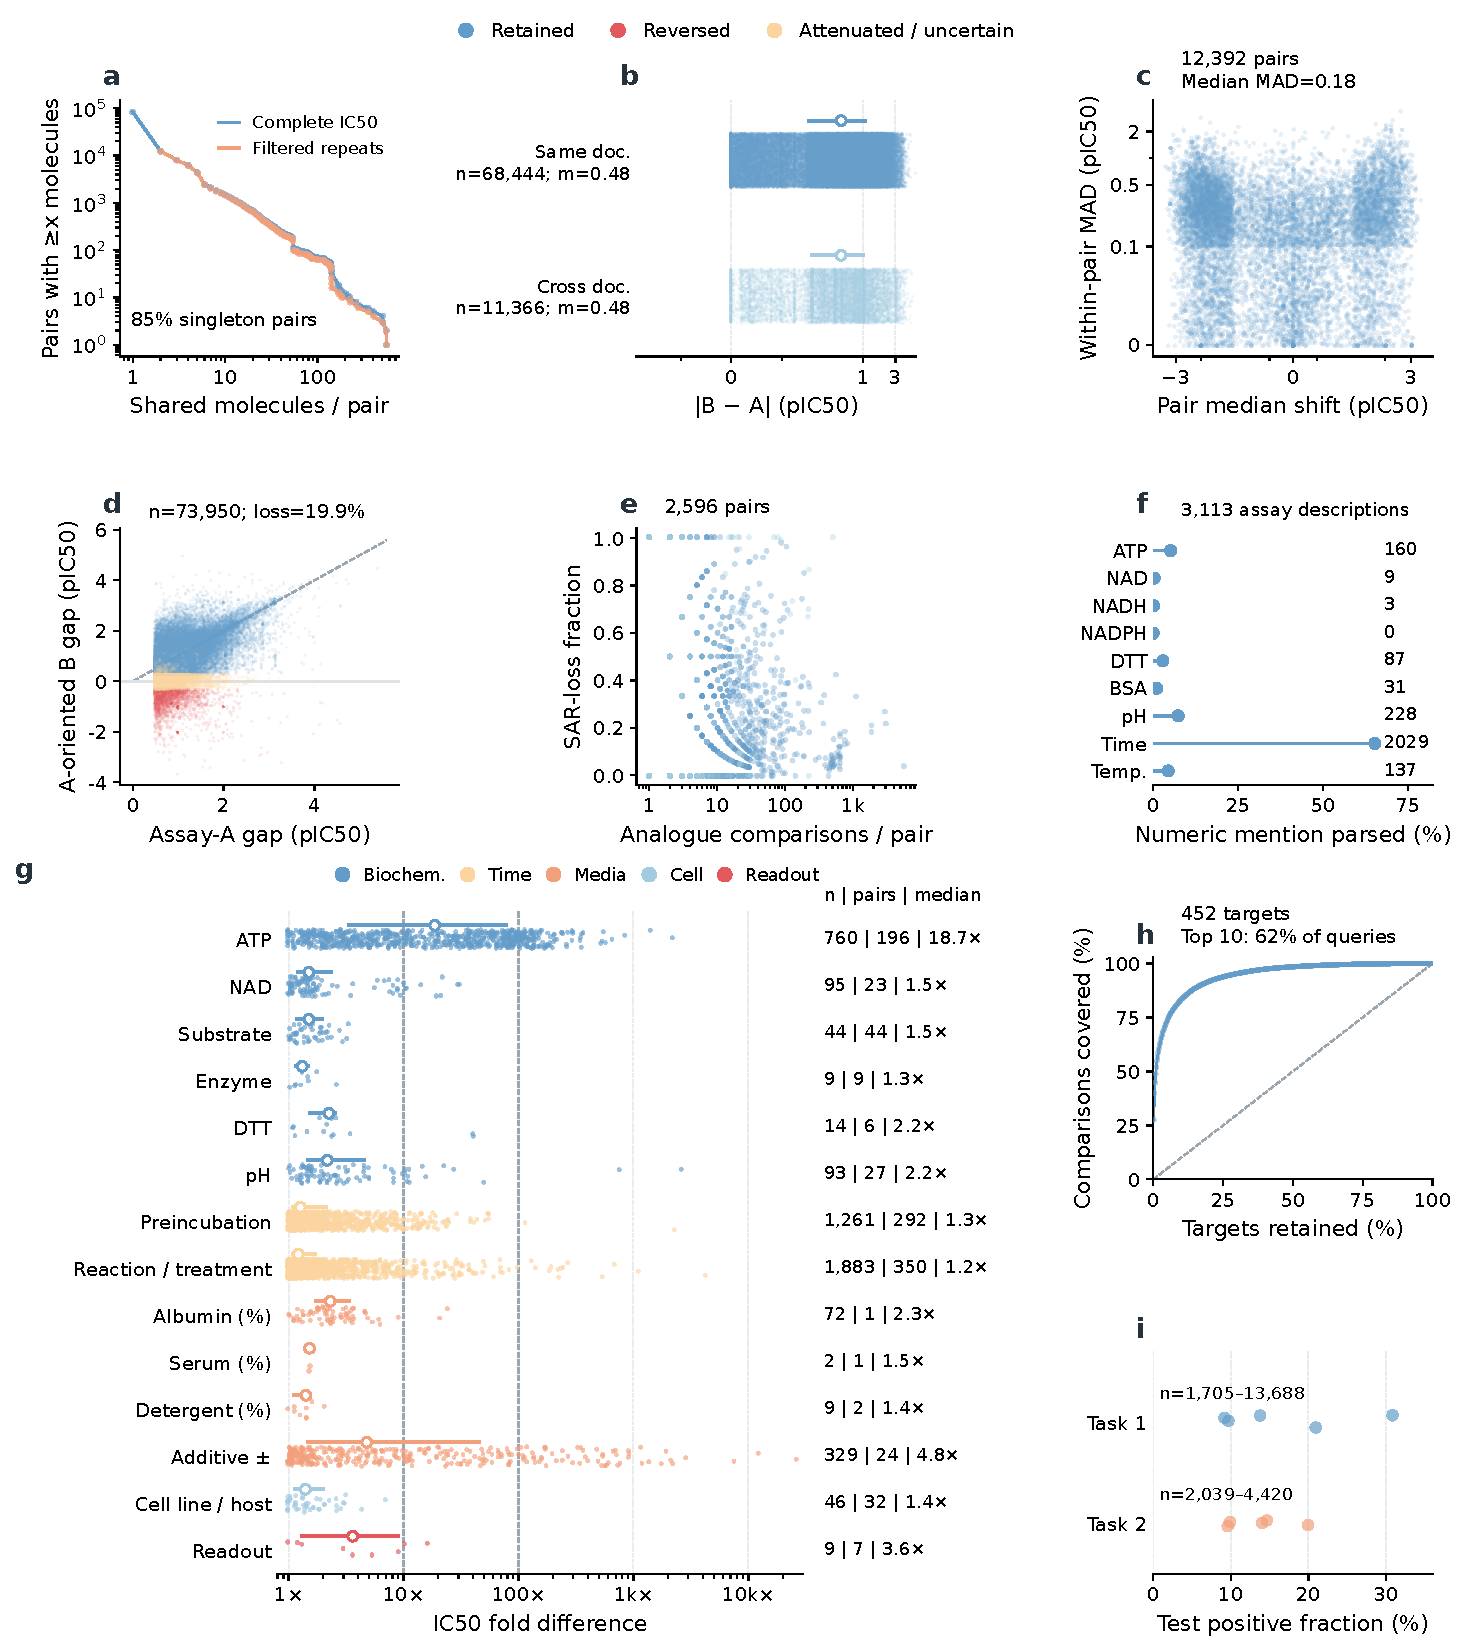
\includegraphics[width=0.98\textwidth,height=0.75\textheight,keepaspectratio]{figure2_data_audit.pdf}
\caption{Dataset support, response heterogeneity and reported-condition coverage. (a) Pair-support survival in the complete IC$_{50}$ resource and filtered repeated-pair pool; 85\% of original pairs are singletons. (b) All 79,810 paired molecular disagreements by document relationship; open circles and intervals give medians and interquartile ranges. (c) Full-pair median shifts and median absolute deviations for 12,392 pairs. These are descriptive statistics; Task 2 fits its centers from training data only. (d) All 73,950 analogue questions, colored by outcome, with assay-B gaps oriented by the assay-A ordering. (e) Comparison support and loss fraction for all 2,596 analogue-supported pairs. (f) Parsed numeric-mention coverage across 3,113 assay descriptions, with observed counts. (g) All 4,626 sample--condition rows from the separate 14-condition audit; row annotations give observations, pairs and median fold differences. Open circles and intervals mark medians and interquartile ranges. (h) Target coverage ranked by comparison count; the largest ten targets contribute 62\% of queries. (i) Test positive fractions for the five fixed seeds, annotated with query-count ranges. Dots are observations, pairs or seeds as specified; repeated records and splits are dependent.}
\label{fig:data}
\end{figure}
\clearpage
\subsection{Prediction performance against baseline methods}

Tables~\ref{tab:baselines-task1}--\ref{tab:baselines-task2} and Figure~\ref{fig:gains} compare baseline methods on identical test queries. For SAR transfer, SAGP reaches AP 0.5395, within-pair AUROC 0.7459 and macro MAE 0.3212. Improvements over threshold-monotone boosting are +0.0443 AP (95\% component interval 0.0128--0.0609) and +0.0257 within-pair AUROC (0.0113--0.0474). These gains support predicting whether an analogue conclusion transfers between the two assays.

For molecular sensitivity, AP is 0.6439, within-pair AUROC 0.6969 and macro MAE 0.1602. Against molecular kNN, differences are +0.0895 AP (95\% CI 0.0462--0.1448), +0.0672 within-pair AUROC (0.0233--0.1047) and $-0.0280$ MAE ($-0.0632$ to $-0.0103$). SAGP has the highest mean AP, global AUROC and within-pair AUROC, together with the lowest mean MAE in Table~\ref{tab:baselines-task2}. The within-pair gain shows that prediction benefits extend beyond identifying assay transitions with high overall event prevalence.

Final-step results are reported in Supplementary Table~\SIFinalTable.

\begin{table}[htbp]
\centering
\caption{Known-pair SAR transfer. Results are mean $\pm$ SD across five fixed scaffold splits.}
\label{tab:baselines-task1}
\small
\setlength{\tabcolsep}{6pt}
\resizebox{\textwidth}{!}{%
\begin{tabular}{lrrrr}
\toprule
Method & AP $\uparrow$ & AUROC $\uparrow$ & Pair AUROC $\uparrow$ & Macro MAE $\downarrow$ \\
\midrule
Constant risk / unchanged A gap & 0.169 $\pm$ 0.091 & 0.500 $\pm$ 0.000 & 0.500 $\pm$ 0.000 & 0.398 $\pm$ 0.031 \\
Logistic regression / ridge & 0.433 $\pm$ 0.136 & 0.760 $\pm$ 0.044 & 0.629 $\pm$ 0.036 & 0.465 $\pm$ 0.058 \\
Random forest & 0.517 $\pm$ 0.151 & 0.830 $\pm$ 0.026 & 0.726 $\pm$ 0.029 & 0.445 $\pm$ 0.062 \\
Within-pair molecular kNN & 0.435 $\pm$ 0.178 & 0.686 $\pm$ 0.103 & 0.552 $\pm$ 0.037 & 0.541 $\pm$ 0.069 \\
Contrast boosting & 0.493 $\pm$ 0.137 & 0.817 $\pm$ 0.031 & 0.713 $\pm$ 0.054 & 0.344 $\pm$ 0.026 \\
Threshold-monotone boosting & 0.495 $\pm$ 0.130 & 0.819 $\pm$ 0.021 & 0.720 $\pm$ 0.057 & -- \\
Direct MLP & 0.436 $\pm$ 0.181 & 0.723 $\pm$ 0.076 & 0.626 $\pm$ 0.032 & 0.506 $\pm$ 0.091 \\
Reference attention & 0.445 $\pm$ 0.180 & 0.735 $\pm$ 0.065 & 0.640 $\pm$ 0.032 & 0.481 $\pm$ 0.085 \\
Neural local empirical Bayes & 0.478 $\pm$ 0.157 & 0.800 $\pm$ 0.044 & 0.693 $\pm$ 0.036 & 0.378 $\pm$ 0.036 \\
\midrule
SAGP (ours) & \textbf{0.539 $\pm$ 0.148} & \textbf{0.844 $\pm$ 0.012} & \textbf{0.746 $\pm$ 0.055} & \textbf{0.321 $\pm$ 0.026} \\
\bottomrule
\end{tabular}}
\par\vspace{3pt}
\begin{minipage}{0.98\textwidth}\footnotesize
Pair AUROC uses the same strict rule for every row: at least ten queries and three per class. Bold marks the largest mean for ranking metrics or the smallest mean error. All methods use identical test IDs and outcomes within each seed. Linear and forest classification/regression estimators address separate endpoints; their outputs are never fused. The threshold classifier has no continuous output; its companion gap regressor is listed under contrast boosting. Training objectives and available reference representations differ.
\end{minipage}
\end{table}

\begin{table}[htbp]
\centering
\caption{Molecular sensitivity within a known assay pair. Results are mean $\pm$ SD across five fixed scaffold splits.}
\label{tab:baselines-task2}
\small
\setlength{\tabcolsep}{6pt}
\resizebox{\textwidth}{!}{%
\begin{tabular}{lrrrr}
\toprule
Method & AP $\uparrow$ & AUROC $\uparrow$ & Pair AUROC $\uparrow$ & Macro MAE $\downarrow$ \\
\midrule
Assay-pair prior & 0.507 $\pm$ 0.032 & 0.865 $\pm$ 0.011 & 0.500 $\pm$ 0.000 & 0.196 $\pm$ 0.033 \\
Logistic regression / ridge & 0.452 $\pm$ 0.080 & 0.831 $\pm$ 0.030 & 0.555 $\pm$ 0.042 & 0.226 $\pm$ 0.036 \\
Random forest & 0.564 $\pm$ 0.046 & 0.878 $\pm$ 0.012 & 0.649 $\pm$ 0.070 & 0.195 $\pm$ 0.031 \\
Within-pair molecular kNN & 0.554 $\pm$ 0.050 & 0.868 $\pm$ 0.008 & 0.630 $\pm$ 0.048 & 0.188 $\pm$ 0.027 \\
XGBoost & 0.457 $\pm$ 0.022 & 0.865 $\pm$ 0.011 & 0.568 $\pm$ 0.030 & 0.197 $\pm$ 0.025 \\
Direct MLP & 0.483 $\pm$ 0.072 & 0.821 $\pm$ 0.047 & 0.583 $\pm$ 0.061 & 0.216 $\pm$ 0.032 \\
Reference attention & 0.510 $\pm$ 0.046 & 0.844 $\pm$ 0.015 & 0.605 $\pm$ 0.039 & 0.208 $\pm$ 0.031 \\
Neural local empirical Bayes & 0.560 $\pm$ 0.057 & 0.879 $\pm$ 0.015 & 0.615 $\pm$ 0.060 & 0.194 $\pm$ 0.030 \\
\midrule
SAGP (ours) & \textbf{0.644 $\pm$ 0.042} & \textbf{0.898 $\pm$ 0.005} & \textbf{0.697 $\pm$ 0.038} & \textbf{0.160 $\pm$ 0.011} \\
\bottomrule
\end{tabular}}
\par\vspace{3pt}
\begin{minipage}{0.98\textwidth}\footnotesize
Pair AUROC uses the same strict rule for every row: at least ten queries and three per class. Bold marks the largest mean for ranking metrics or the smallest mean error. All methods use identical test IDs and outcomes within each seed. Linear and forest classification/regression estimators address separate endpoints; their outputs are never fused. Training objectives and available reference representations differ.
\end{minipage}
\end{table}

\clearpage
\begin{figure}[p]\centering
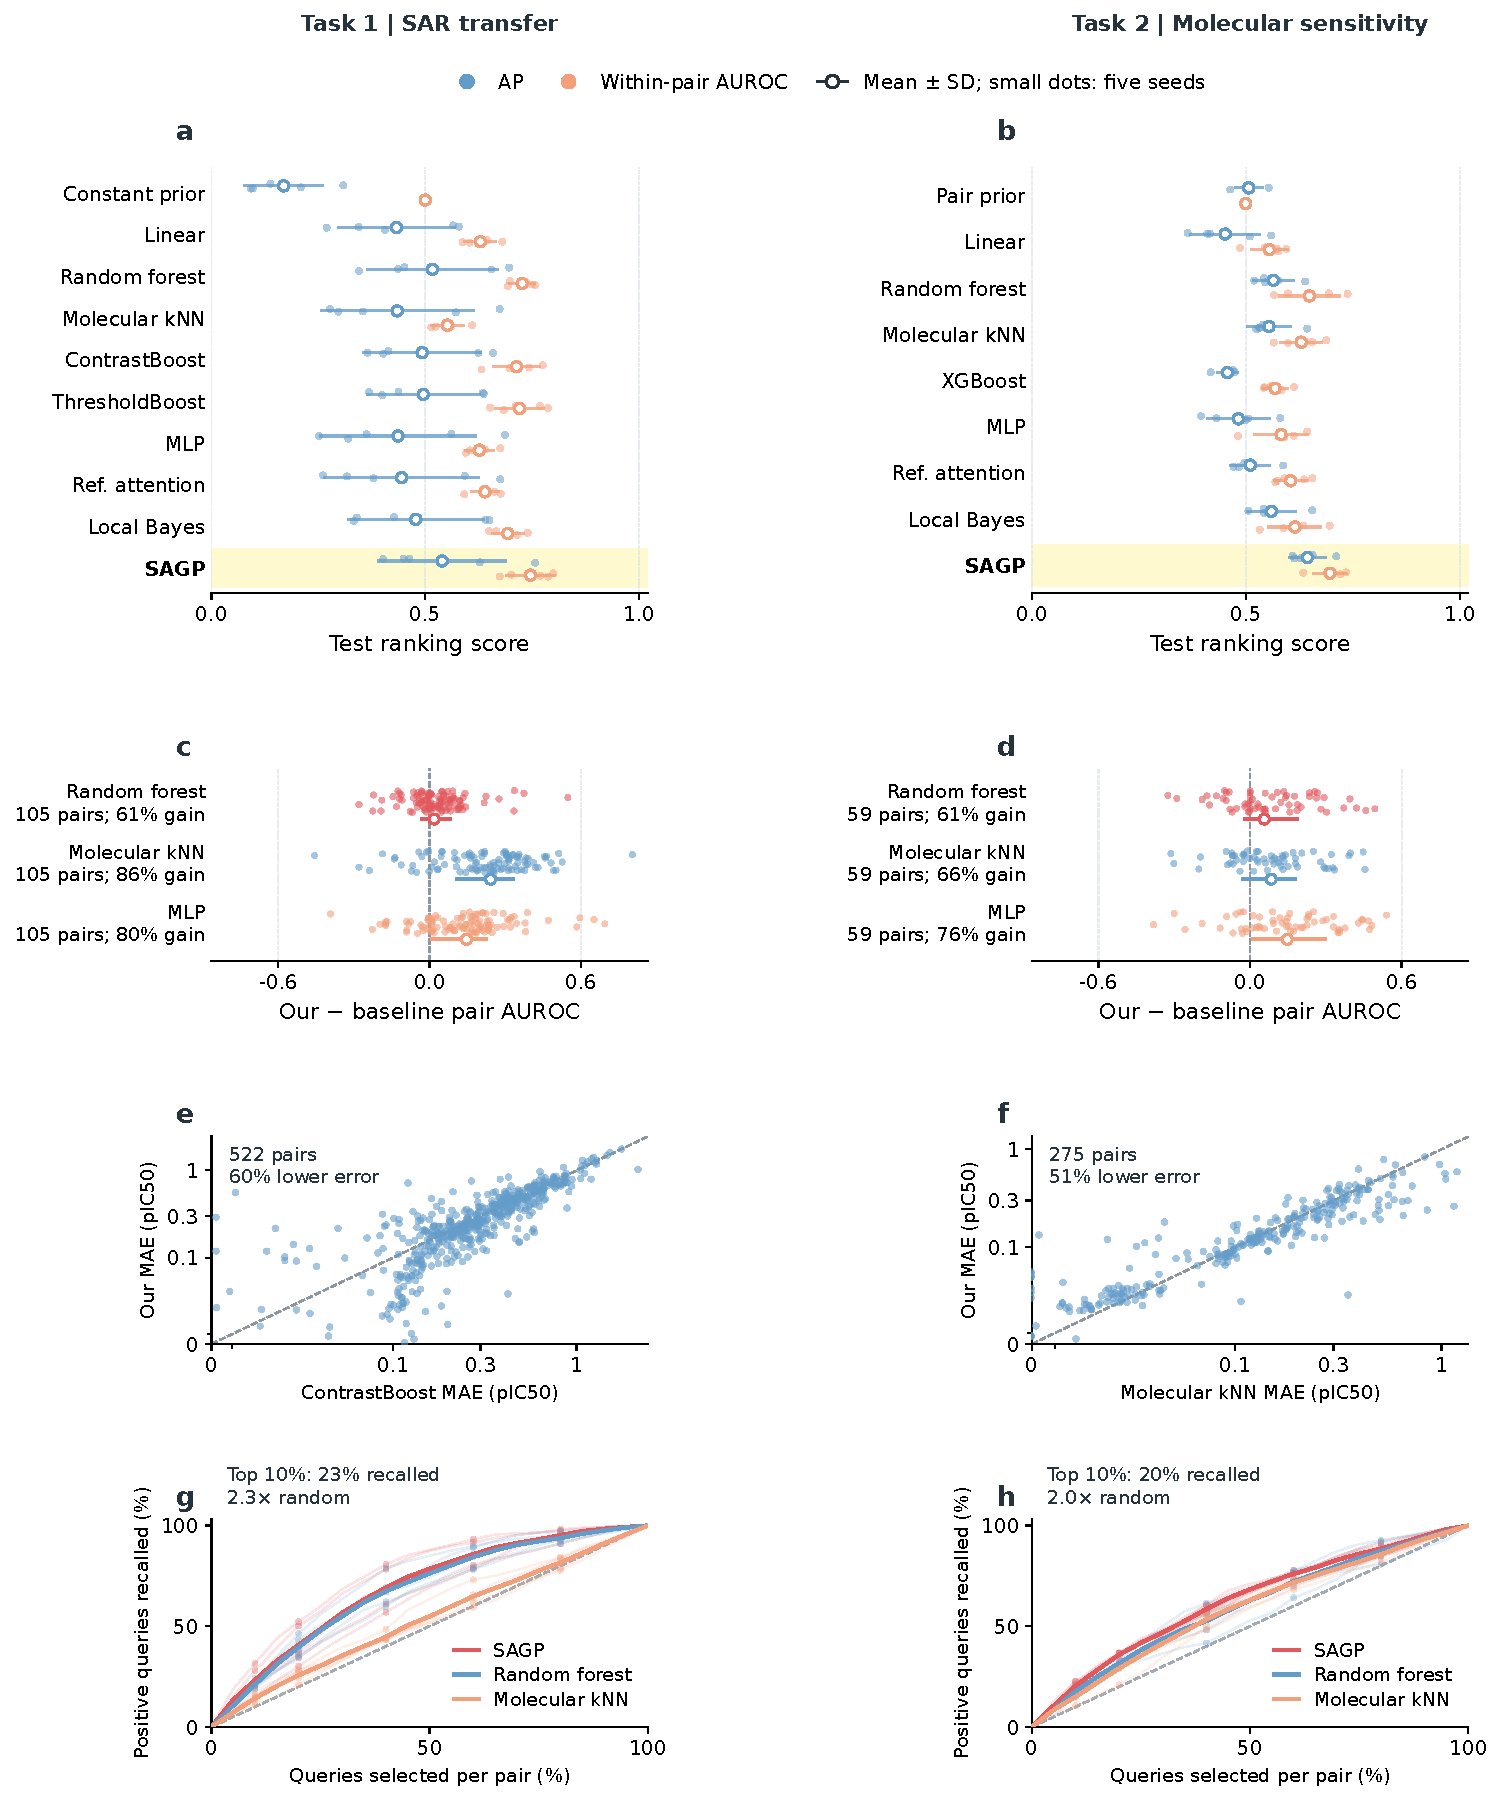
\includegraphics[width=0.98\textwidth,height=0.82\textheight,keepaspectratio]{figure3_model_gains.pdf}
\caption{Baseline comparisons for Tasks 1 and 2. (a,b) AP and within-pair AUROC for the baseline methods, with five split points and mean $\pm$ SD. (c,d) Unique-pair AUROC differences against random forest, molecular kNN and a direct MLP; negative differences are retained. (e,f) Pair MAEs against contrast boosting (Task 1) and molecular kNN (Task 2). (g,h) Positive-query recall under within-pair query selection for SAGP, random forest and molecular kNN. Pair AUROC and recall use the same class-support rule. Pair-level points summarize available splits and are not independent replicates.}
\label{fig:gains}\end{figure}\clearpage
\subsection{Retrospective molecular illustrations}
Figure~\ref{fig:cases} presents retrospectively selected successful examples from both tasks in scaffold split 17. These illustrations explain the prediction outputs; they are not additional independent validation. Task~1 examples are assay-defined analogue pairs; Task~2 examples are individual molecules evaluated by their departure from the training-only assay-pair median. Each scatter shows the full held-out cohort for the displayed pair. The highlighted compounds illustrate retained or reversed SAR and small or large molecular sensitivity, while the complete cohorts also expose prediction errors.

For Task~1, the CHEMBL288 analogue pair retains its assay-A ordering: the observed and predicted A-oriented assay-B gaps are $+1.620$ and $+1.621$ pIC$_{50}$, with predicted SAR-loss probability 0.024. The CHEMBL237 pair reverses its ordering; its observed and predicted oriented gaps are $-1.000$ and $-0.952$ pIC$_{50}$, with predicted loss probability 0.981. The corresponding pair cohorts contain 29 and 38 held-out comparisons. Structures and measured assay potencies are shown in the figure.

For Task~2, the two ROCK2 compounds have observed sensitivities of 0.291 and 0.678 pIC$_{50}$, with predictions of 0.285 and 0.731; cohort MAE is 0.106 over 13 molecules. For estrogen receptor $\beta$, the observed values are 0.326 and 1.300, and predictions are 0.457 and 1.335; cohort MAE is 0.337 over 16 molecules. For ALDH1A1, observed values are 0.372 and 0.707, and predictions are 0.440 and 0.680; cohort MAE is 0.268 over 20 molecules. AUROC values for these complete cohorts are 0.825, 0.844 and 0.835, respectively. Raw assay potencies and compound identifiers are reported in Table~\ref{tab:caseprovenance}.

\begin{figure}[p]
\centering
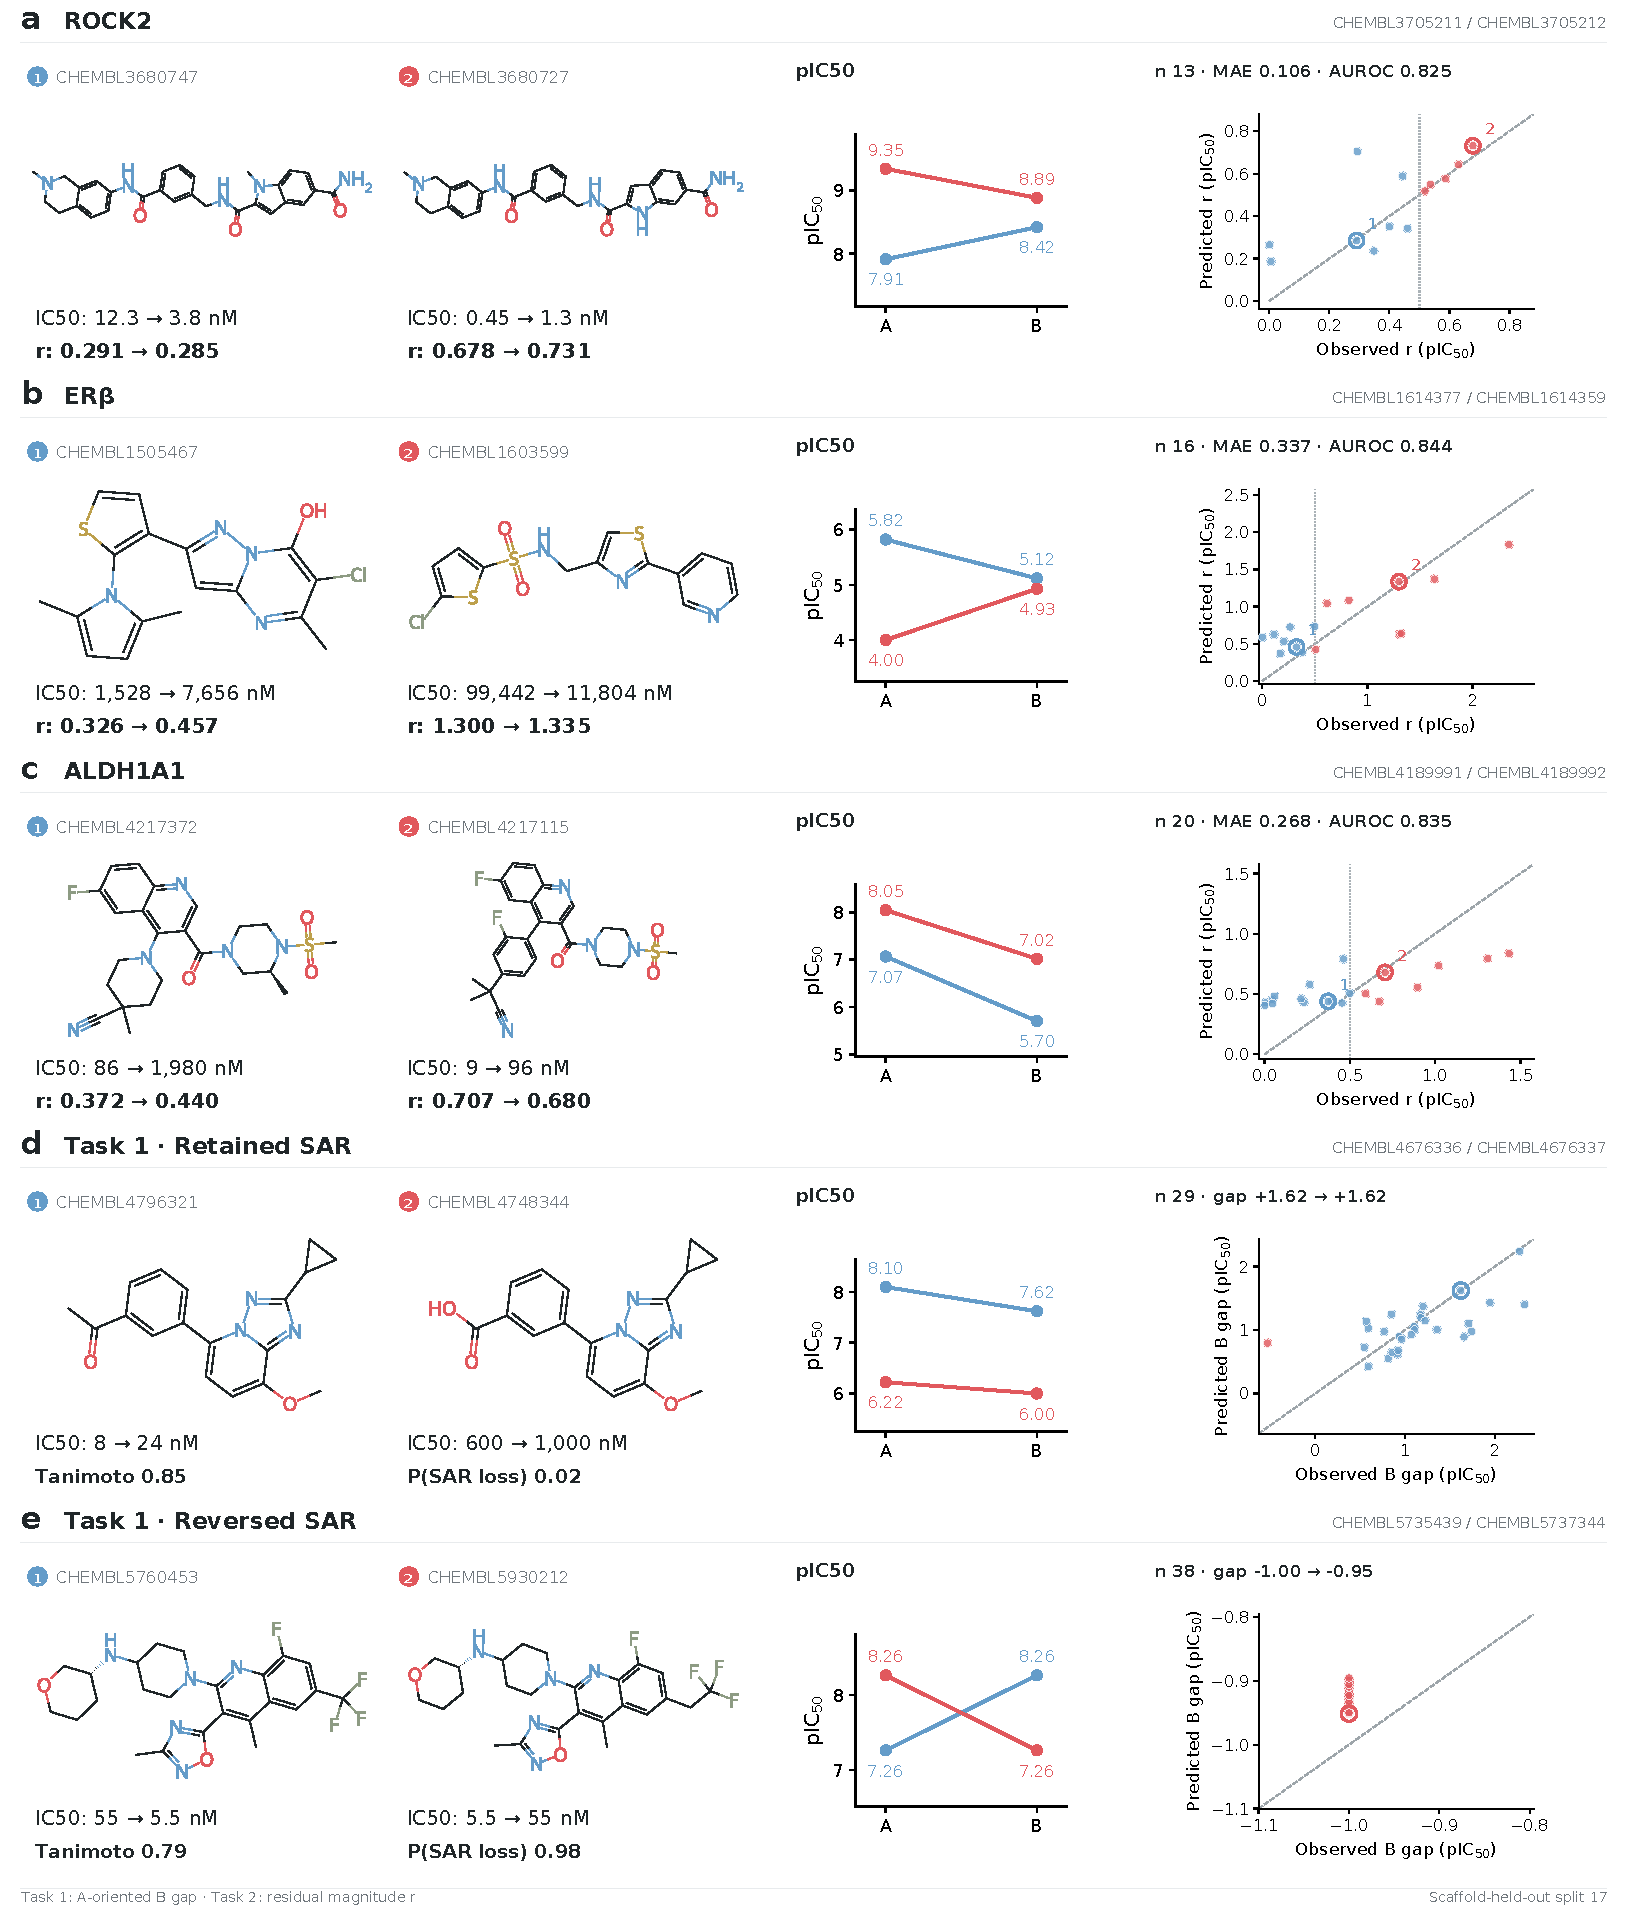
\includegraphics[width=0.98\textwidth,height=0.88\textheight,keepaspectratio]{figure4_casebook.pdf}
\caption{Retrospectively selected molecular illustrations in scaffold split 17. (a--c) Task~2: activity-linked structures, measured assay-A/B potencies, and complete assay-pair test-cohort sensitivity predictions for ROCK2, ER$\beta$ and ALDH1A1. Numbered compounds match the highlighted scatter points. (d,e) Task~1: two matched analogue pairs with retained and reversed SAR, their measured potency tracks, and complete selected-pair test-cohort predictions. B gaps are oriented by the assay-A ordering; the ring highlights the displayed analogue comparison.}
\label{fig:cases}
\end{figure}

\begin{table}[htbp]
\centering
\caption{Measured potencies and held-out residual predictions for the displayed Task~2 compounds. Error is absolute difference in pIC$_{50}$ units; compound identifiers link to source structures.}
\label{tab:caseprovenance}
\small
\begin{tabular}{@{}llrrrrr@{}}
\toprule
Target & Compound & A (nM) & B (nM) & Obs. $r$ & Pred. $r$ & Error \\
\midrule
ROCK2 & CHEMBL3680747 & 12.3 & 3.8 & 0.291 & 0.285 & 0.006 \\
ROCK2 & CHEMBL3680727 & 0.45 & 1.3 & 0.678 & 0.731 & 0.053 \\
ER $\beta$ & CHEMBL1505467 & 1.53e+03 & 7.66e+03 & 0.326 & 0.457 & 0.131 \\
ER $\beta$ & CHEMBL1603599 & 9.94e+04 & 1.18e+04 & 1.300 & 1.335 & 0.036 \\
ALDH1A1 & CHEMBL4217372 & 86 & 1.98e+03 & 0.372 & 0.440 & 0.067 \\
ALDH1A1 & CHEMBL4217115 & 9 & 96 & 0.707 & 0.680 & 0.027 \\
\bottomrule
\end{tabular}
\end{table}

\clearpage

\subsection{Why historical molecular responses help}

Table~\ref{tab:reference-interventions} and Figure~\ref{fig:reference-evidence} evaluate reference dependence with fitted weights and test queries fixed. Increasing the cap from 3 to 100 references raises SAR-transfer AP from 0.3712 to 0.5395 and sensitivity AP from 0.4442 to 0.6439; sensitivity within-pair AUROC rises from 0.6240 to 0.6969 and macro MAE falls from 0.2167 to 0.1602. Full-cap versus three-reference differences have component intervals excluding zero for both tasks' AP, within-pair AUROC and MAE. Most SAR-transfer AP improvement is already present by 30 references. Sensitivity magnitude continues to benefit from additional references, although gains become smaller.

Shuffling historical signed responses within each pair lowers sensitivity AP to 0.4548 and within-pair AUROC to 0.5270, while macro MAE rises to 0.2112. SAR-transfer AP falls to 0.3304 and within-pair AUROC to 0.7086. Intact-minus-shuffled within-pair AUROC differences are 0.0373 (95\% CI 0.0126--0.0596) for SAR transfer and 0.1699 (0.1133--0.2193) for sensitivity. The intervention preserves the pair's marginal response distribution while breaking its correspondence with molecular structure. Historical molecule--response associations therefore provide useful information beyond an assay-wide shift distribution. This result does not establish that the model identifies the causal contribution of any particular experimental condition.

The reference-budget experiment measures information use during prediction. Because sensitivity labels and their median offset retain the complete training pool, it does not establish the accuracy achievable after collecting only three or ten measurements in a new assay. Its practical implication is that a supported transition benefits from retaining the identities and responses of previously measured compounds.

Response-component distributions in Figure~\ref{fig:reference-evidence}g--i compare event retrieval, within-pair ranking and magnitude accuracy across five scaffold evaluations. Task 1 and Task 2 are displayed separately. Their differing trends show why molecular ranking and numerical sensitivity should be evaluated together; improvements on one endpoint do not imply improvements on all endpoints.

\begin{table}[htbp]\centering\small
\caption{Frozen reference interventions. Mean $\pm$ SD over five dependent scaffold splits.}
\label{tab:reference-interventions}
\resizebox{\textwidth}{!}{%
\begin{tabular}{llrrr}\toprule
Task & Reference cap / control & AP & Pair AUROC & Macro MAE\\\midrule
1 & 3 & 0.3712 $\pm$ 0.1301 & 0.7275 $\pm$ 0.0556 & 0.3726 $\pm$ 0.0185\\
2 & 3 & 0.4442 $\pm$ 0.0550 & 0.6240 $\pm$ 0.0614 & 0.2167 $\pm$ 0.0306\\
1 & 10 & 0.4944 $\pm$ 0.1545 & 0.7295 $\pm$ 0.0569 & 0.3421 $\pm$ 0.0196\\
2 & 10 & 0.5540 $\pm$ 0.0493 & 0.6429 $\pm$ 0.0523 & 0.1886 $\pm$ 0.0216\\
1 & 30 & 0.5360 $\pm$ 0.1477 & 0.7379 $\pm$ 0.0533 & 0.3265 $\pm$ 0.0224\\
2 & 30 & 0.6253 $\pm$ 0.0384 & 0.6760 $\pm$ 0.0335 & 0.1664 $\pm$ 0.0154\\
1 & 100 & 0.5395 $\pm$ 0.1481 & 0.7459 $\pm$ 0.0554 & 0.3212 $\pm$ 0.0257\\
2 & 100 & 0.6439 $\pm$ 0.0422 & 0.6969 $\pm$ 0.0384 & 0.1602 $\pm$ 0.0114\\
1 & Shuffled response, 100 & 0.3304 $\pm$ 0.0888 & 0.7086 $\pm$ 0.0602 & 0.4003 $\pm$ 0.0379\\
2 & Shuffled response, 100 & 0.4548 $\pm$ 0.0445 & 0.5270 $\pm$ 0.0334 & 0.2112 $\pm$ 0.0315\\
\bottomrule\end{tabular}}
\par\vspace{3pt}\begin{minipage}{0.96\textwidth}\footnotesize Caps are maximum available reference counts. Weights, queries and labels stay fixed; Task 2 retains its full-training-pool median offset. One nested support order and one within-pair response shuffle are evaluated per split. SD is not a confidence interval. All controls and all unfavorable outcomes are retained.\end{minipage}
\end{table}

\clearpage
\begin{figure}[p]\centering
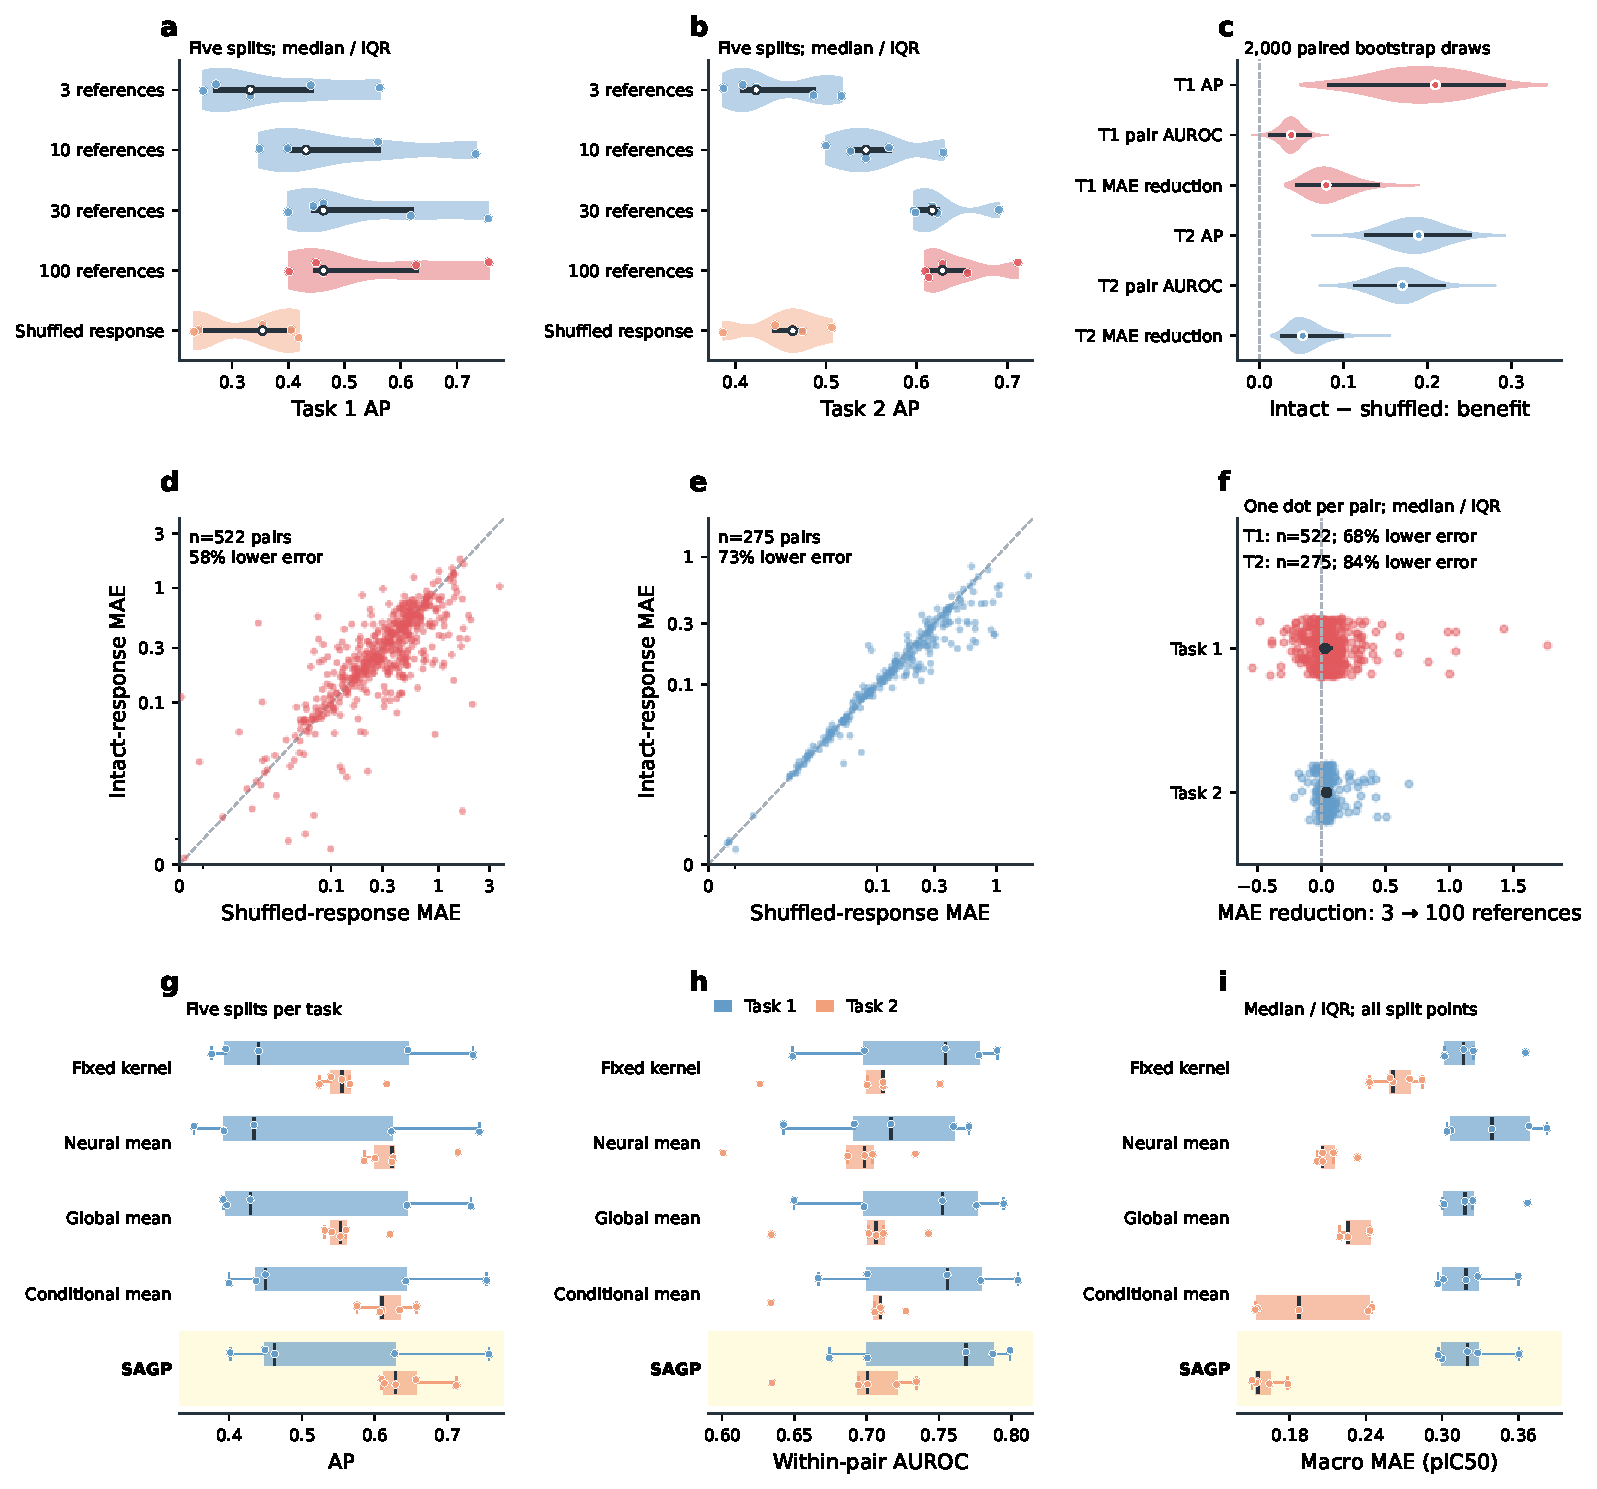
\includegraphics[width=\textwidth,height=0.78\textheight,keepaspectratio]{figure5_reference_evidence.pdf}
\caption{Historical reference evidence and SAGP response analysis. (a,b) AP at nested reference caps and the shuffled-response control: violin densities of five scaffold evaluations, with all split points, median and IQR. (c) Intact-minus-shuffled benefits: violin densities of 2,000 paired component-bootstrap draws, with the original estimate and percentile 95\% interval. (d,e) Pair MAEs under intact versus shuffled responses. (f) Pair MAE reductions from 3 to 100 references, with median and IQR. Pair points average available splits; Task 2 labels and offsets retain the full training pool. (g--i) AP, within-pair AUROC and macro MAE for five response formulations. Blue: Task 1; peach: Task 2. Each box summarizes five scaffold evaluations: median, interquartile range and whiskers extending to observations within 1.5 IQR; all split observations are overlaid. Formulations use the same test queries but differ in training objectives.}
\label{fig:reference-evidence}\end{figure}\clearpage

\subsection{Reliability, applicability and data limitations}

Figure~\ref{fig:applicability} separates numerical accuracy from probability reliability. Retaining the globally lowest-variance 20\% of queries reduces SAR-transfer micro MAE from 0.3400 to 0.1837 and sensitivity micro MAE from 0.1464 to 0.0760. When the same nominal fraction is retained within every assay pair, macro MAE changes only from 0.3212 to 0.3046 and from 0.1602 to 0.1526, respectively. Much of the global selective gain consequently depends on changing the mixture of assay pairs. Uncertainty-based selection offers a smaller improvement when the transition is held fixed, and it should be assessed in the intended prioritization setting.

Sensitivity risks have mean Brier score 0.0757, log loss 0.2478 and ECE 0.0279; SAR-transfer ECE is 0.0444. Pair-level observed rates nevertheless vary around the predicted rates. A low query-level calibration error does not guarantee accurate probabilities for each assay transition. Moreover, some controls have better individual reliability metrics: the unadjusted Gaussian probability has sensitivity Brier score 0.0750, while its SAR-transfer ECE is 0.0399. Discrimination, magnitude error and calibration therefore capture different aspects of utility.

Outside the training-defined ten most frequent targets, within-pair AUROC is 0.7160 for SAR transfer and 0.7046 for sensitivity, but macro MAE increases to 0.4078 and 0.2241. Ranking remains useful in that subset while numerical accuracy is weaker. Severe sensitivity events are easier to rank globally than milder departures: AUROC rises from 0.8503 at a 0.3 pIC$_{50}$ threshold to 0.9501 at 1.0. Those thresholds define different event populations; they do not imply equal performance for every assay pair.

The most favorable use is a known transition with enough historical co-measurements to characterize its response. Sparse support, target concentration, same-document dominance and incomplete protocol annotation restrict the evaluated domain. The present data do not validate transfer to entirely new assay pairs, unknown targets or prospectively collected experimental systems. Historical-response evidence can support chemical risk prioritization within represented transitions, while ambiguous predictions still require matched experimental measurements.

\begin{figure}[p]\centering
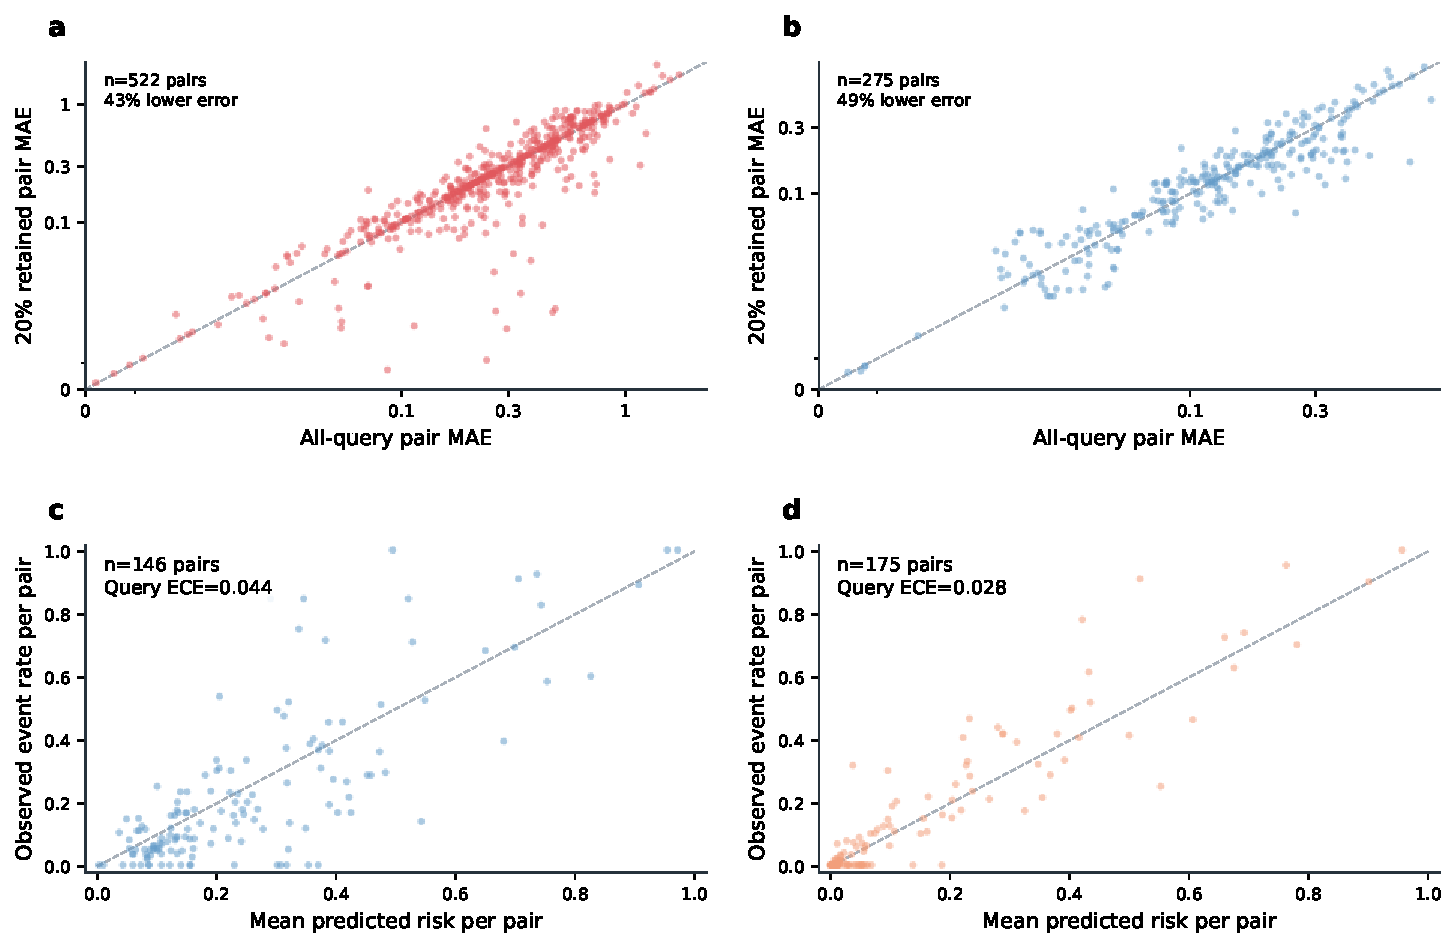
\includegraphics[width=\textwidth,height=0.78\textheight,keepaspectratio]{figure6_applicability_reliability.pdf}
\caption{Selective error and probability reliability: left, Task 1; right, Task 2. (a,b) Mean available-split MAE for each unique assay pair using all queries versus its 20\% lowest-variance queries, retaining at least one query per pair. (c,d) Pair-mean predicted risk versus observed event rate, for pairs with at least ten queries in a split. The diagonal indicates equal rates. Annotated ECE separately uses all query probabilities. Symmetric logarithmic error axes retain zero and extreme points. Pair points average available eligible splits.}
\label{fig:applicability}\end{figure}\clearpage

\section{Conclusions}

We define two source-traceable prediction problems within known assay pairs: whether a robust analogue ordering transfers between assays, and how strongly an individual molecule departs from their common shift. This separates the reliability of a relative chemical conclusion from the sensitivity of an individual compound.

Historical molecule--response correspondence contains predictive information beyond the assay-wide shift distribution, as demonstrated by reference-response shuffling. SAGP improves sensitivity and transfer predictions over molecular and empirical baseline methods. The response analyses show that different endpoints benefit differently from representing shared assay trends and local chemical variation.

The intended setting is an assay transition with a useful history of compounds measured in both systems. Predictions can help prioritize SAR-transfer risk and unusually sensitive molecules for review. Generalization to new assay pairs or unknown targets, and reductions in experimental cost, remain questions for future prospective evaluation.

\section{Implementation and reproducibility}

SAGP was implemented in Python using PyTorch and RDKit. Supplementary Methods and the repository README provide the software environment, key hyperparameters, checkpoint-selection rule and commands for reproducing training, evaluation and figures.

\section{Data and Software Availability}

The original bioactivity data were obtained from ChEMBL release 37 (\url{https://doi.org/10.6019/CHEMBL.database.37}). The curated benchmark, five scaffold splits and reference selections, together with SAGP source code, trained model files, per-query predictions, figure source data and reproduction scripts, are publicly available in repository version \texttt{v1.0.1}. The original ChEMBL database is downloaded separately from EMBL--EBI; ChEMBL-derived data retain the Creative Commons Attribution--ShareAlike 3.0 license. Repository files can be downloaded without registration or access approval. The manuscript-aligned version is identified by the \texttt{v1.0.1} tag at \url{https://github.com/jiajunyu1999/SAGP}.

\bibliographystyle{plainnat}
\bibliography{references}
\end{document}
